\subsubsection{Descrizione generale}
Questo servizio implementa le funzionalità di scraping\G{} ed in generale ottenimento dati da Instagram\G{} e altre piattaforme ad esso correlate.

\subsubsection{Diagramma delle classi}
\begin{figure}[H]
    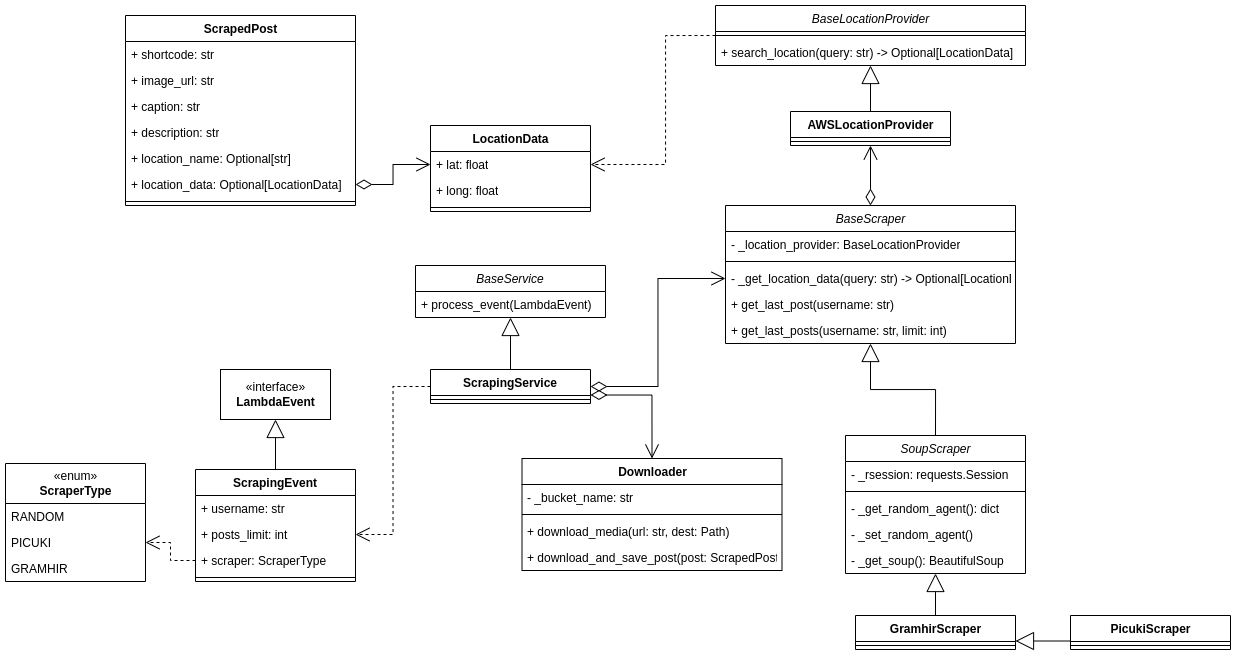
\includegraphics[width=15cm]{sezioni/images/cd_scraping.png}
    \centering
    \caption{Scraping Service - Diagramma delle classi}
\end{figure}

\subsubsection{Diagramma di sequenza}
\begin{figure}[H]
    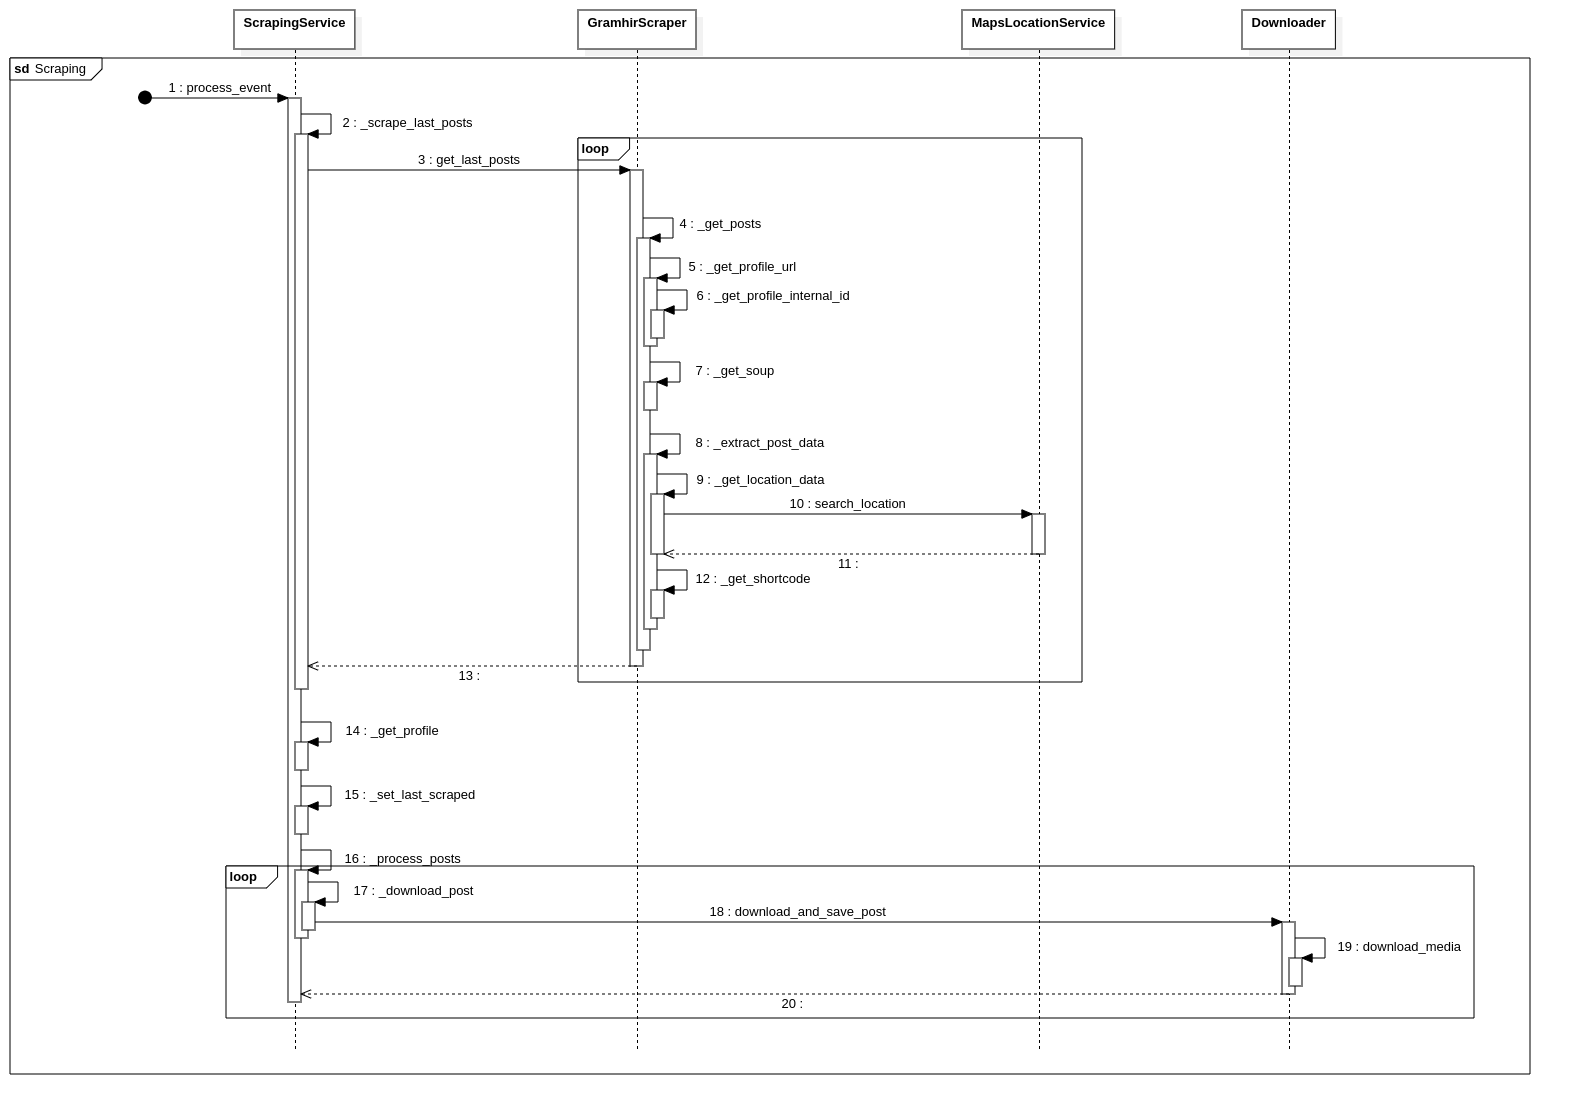
\includegraphics[width=15cm]{sezioni/images/sd_scraping.png}
    \centering
    \caption{Scraping Service - Diagramma di sequenza}
\end{figure}

\subsubsection{Schemi I/O}
\paragraph*{Input} esempio di evento in input, in formato JSON\G{}.
\begin{lstlisting}[language=JSON]
{
    "username": "antoniorazzi",
    "posts_limit": 10
}
\end{lstlisting}
Descrizione:
\begin{itemize}
    \item \verb|username|: username del profilo social da cui effettuare lo scraping\G;
    \item \verb|posts_limit|: numero massimo di post di cui effettuare lo scraping\G. 
\end{itemize}

\paragraph*{Output} esempio di risposta in output, in formato JSON\G{}.
\begin{lstlisting}[language=JSON]
{
    "posts_count": 2,
    "posts": [
        {"id": 4},
        {"id": 5}
    ]
}
\end{lstlisting}
Descrizione:
\begin{itemize}
    \item \verb|posts_count|: numero di post ottenuti;
    \item \verb|posts|: array di post. 
\end{itemize}

\subsubsection{Strategie di scraping}
Le azioni di scraping\G{} non avvengono direttamente su Instagram\G, questo perchè comporterebbe il
rischio di incorrere in \textit{rate limiting} o addirittura l'impossibilità totale di usufruire del servizio dall'infrastruttura cloud di AWS\G.
Per aggirare queste problematiche, lo scraping\G{} avviene da piattaforme chiamate \textit{viewer},
che propongono in larga parte gli stessi contenuti di Instagram\G, ma in un formato molto più semplice da trattare automaticamente.\aCapo
Le classi \verb|SoupScraper| e più in generale \verb|BaseScraper|, si occupano di fornire interfacce comuni per gli scraper\G{} che andranno implementati.
Le classi \verb|GramhirScraper| e \verb|PicukiScraper| si occupano di effettuare lo scraping 
rispettivamente dai viewer \textit{Gramhir} (\url{https://www.gramhir.com}) e \textit{Picuki} (\url{https://www.picuki.com}). Gli algoritmi e le tecniche utilizzate dalle due classi, sono sostanzialmente identiche.
Infatti, \verb|PicukiScraper| eredita direttamente da \verb|GramhirScraper|.
Il funzionamento interno delle due piattaforme differisce solo nella necessità di ottenere un 
\textit{ID} correlato al profilo social che si vuole visualizzare, necessario per \textit{Gramhir}.

\begin{lstlisting}[language=Python, caption=Ottenimento URL profilo in \textit{Gramhir}]
def _get_profile_url(self, username: str) -> str:
    gramhir_id = self._get_profile_internal_id(username)
    profile_url = self._PROFILE_URL.format(username=username, gramhir_id=gramhir_id)
    return profile_url
\end{lstlisting}

\begin{lstlisting}[language=Python, caption=Ottenimento URL profilo in \textit{Picuki}]
def _get_profile_url(self, username: str) -> str:
    return self._PROFILE_URL.format(username=username)
\end{lstlisting}

\aCapo{}
Lo scraping vero e proprio avviene tramite parsing\G{} del contenuto HTML\G{} delle pagine web
fornite dai \textit{viewer}.
\begin{lstlisting}[language=Python, caption=Estrazioni dati tramite parsing\G{}]
def _extract_post_data(self, post_result: Tag) -> ScrapedPost:
    location_name = post_result.find(attrs={'class': 'photo-location'}).get_text(
        strip=True
    )
    location_name = location_name if location_name else None

    location_data = None
    if location_name:
        location_data = self._get_location_data(location_name)

    details_url = post_result.find('a').get('href')
    shortcode = self._get_shortcode(details_url)

    return ScrapedPost(
        image_url=post_result.find('img').get('src'),
        caption=post_result.find(attrs={'class': 'photo-description'}).get_text(
            strip=True
        ),
        description='',
        location_name=location_name,
        location_data=location_data,
        shortcode=shortcode,
    )
\end{lstlisting}

\subsubsection{Ottenimento informazioni relative alle posizioni}
Correlare i post ottenuto a precise posizioni reali è necessario ai fini del progetto.
I dati relativi alla posizione, nelle piattaforme sopracitate, comprendono solo il nome del
particolare punto di interesse, non le coordinate esatte in latitudine e longitudine.
Per estrapolare questi due valori, viene utilizzato il servizio \textit{Google Maps API}\G.\aCapo{}
La classe \verb|MapsLocationProvider|, che concretizza \verb|BaseLocationProvider|, ha il compito
di ottenere informazioni specifiche relative ad un punto di interesse, a partire dal nome.

\begin{lstlisting}[language=Python, caption=Ottenimento informazioni da \textit{Google Maps API}]
def search_location(self, query: str) -> Optional[LocationData]:
    geocode_result = self._maps.geocode(query)

    if not geocode_result:
        return None

    geocode_result = geocode_result[0]
    coords = geocode_result['geometry']['location']
    maps_place_id = geocode_result.get('place_id')

    place = self._maps.place(place_id=maps_place_id)
    address = place['result']['formatted_address']
    name = place['result']['name']
    types = place['result']['types']

    return LocationData(
        lat=coords['lat'],
        long=coords['lng'],
        address=address,
        maps_name=name,
        maps_place_id=maps_place_id,
        types=types
    )
\end{lstlisting}
    

\subsubsection{Salvataggio dei dati}
I dati relativi ai post ottenuti e le relative posizioni, vengonono salvati nel database.
Le immagini o altri contenuti multimediali vengonono salvati nell'apposito bucket\G in S3.
